\documentclass[12pt]{article}
%\usepackage[dvips]{graphicx,lscape}
\usepackage{amsmath}
\usepackage{amssymb}
\usepackage{tikz}
%\usepackage{chicago}

 %\renewcommand{\rmdefault}{cmss}
 %\usepackage{sansmath}
 %\sansmath

\setlength{\textwidth}{6.5in} \setlength{\topmargin}{-0.5in}
\setlength{\textheight}{9.25in} \setlength{\evensidemargin}{0in}
\setlength{\oddsidemargin}{0in}

\newcommand{\NNN}{\mathbb{N}}
\newcommand{\calP}{{\mathcal P}}
\newcommand{\QQQ}{\mathbb{Q}}
\newcommand{\CCC}{\mathbb{C}}
\newcommand{\DDD}{\mathbb{D}}
\newcommand{\RRR}{\mathbb{R}}
\newcommand{\TTT}{\mathbb{T}}
\newcommand{\ZZZ}{\mathbb{Z}}
\newcommand{\st}{\,:\,}

\parindent 0pt

\parskip 3mm

\begin{document}

\newcommand{\bs}{\boldsymbol}
\newcommand{\Cov}{\text{Cov}}


\section*{Some random notes, remarks and observations}

\begin{itemize}

\item `Most' graphs on $n$ vertices have about $\frac{1}{2} \binom{n}{2} \approx \frac{n^2}{4}$ edges.

\item If edges are chosen with probability $p$ then we will average $p \binom{n}{p}$ edges, with a variance of $p(1-p) \binom{n}{2}$. The standard deviation is therefore smaller than $\sqrt{\frac{n^2}{8}} \approx 0.35 n$.  When $n$ gets at all large different values of $p$ will give measures of effectively disjoint support.

\item the `typical' mgr seems to be closely related to the number of edges.  At the endpoints we get
   \begin{itemize}  %[label=$*$]
     \item[$*$] $edges = n-1$, gives $mgr > 1$.
     \item[$*$] $edges = \binom{n}{2}$ gives $mgr = \infty$.
   \end{itemize}
   In the middle the typical mgrs seem to cluster into a smaller and smaller range, whose mean is going to zero. This is presumably because a large graph with a middling number of edges will almost surely have a certain bipartite graph inside it.

\item Experimentally, the observed mgrs from random graphs ($p = 0.5)$ are completely disjoint from the graphs with very small or a very large number of edge

\item You can get a large mgr by joining together two smaller graphs with large mgr's with a single edge (or at a single point). In particular you can join together to complete graphs $K_m$. For these graphs you can often explicitly write down an expression for $\mathrm{det}(D_p)$ and $\langle D_p^{-1} 1,1 \rangle$. As $n \to \infty$ these expressions become even simpler and you can calculate the limiting value. For example, if you take an even value of $n$ and let $G$ be two $K_{n/2}$ graphs joined by a single edge, then the mgr is given by the sum of entries test, which boils down to solving (details omitted!)
    \begin{multline*} (n-2)(n-4)\cdot 2^p-(\frac{n}{2}-1)(n-2)\cdot 3^p-(\frac{n}{2}-1)(2n-5)\cdot 4^p+(\frac{n}{2}-1)(n-2)\cdot 8^p \\
    +(\frac{n}{2}-1)^2\cdot9^p-(\frac{n}{2}-1)^2\cdot 12^p+n-3= 0.
    \end{multline*}
  If you write $X = 2^p$ and $Y = 3^p$ then this simplifies to solving
  \[ ((X-\frac{Y}{2})n-2X+Y+1)((X^2-2X-Y+2)n-2X^2+4X+2Y-6) = 0.\]
  If you normalize by dividing by $n^2$ and then let $n \to \infty$ you are left with
    \[ (2X-Y)(X^2-2X-Y+2) = 0.\]
  Replacing $X$ and $Y$ and solving this tells you that as $n$ gets large you should get that the mgr should approach
    \[ \frac{1}{\log_2{3}-1} \approx 1.709511\]
  and this is indeed what you see when you calculate the mgrs (by $n=20$ it is correct to this number of digits.

\end{itemize}

\vfill\eject

\section*{Bounds}

The proof in my talk shows that for all $\epsilon > 0$, $\delta \in (0,1)$ there exists $N$ such that if $n \ge N$ then $P\bigl(mgr(X) < \epsilon \,:\, X \in G(n,p)\bigr) > 1-\delta$. The proof is `effective' in that you can calculate a value of $N(\epsilon,\delta)$, but the proof is so sloppy that the bound is insane. (Doing a few rough estimates I got something like\footnote{The $10^{5/\epsilon^2}$ term is really $2^{-\binom{2m}{2}}\binom{2m-1}{m}$ which VERY roughly appears to be of order $10^{-m^2/2}$.} $N(\epsilon,\delta) \precapprox \frac{6}{\epsilon} \log\big( \frac{1}{\delta}\bigr)\, 10^{5/\epsilon^2}$.)

The main point is that if $m > \frac{3}{\epsilon}$ then $\log_2(1+\frac{1}{m-1}) < \epsilon$ and so if $K_{m,m}$ sits inside $X$, then $mgr(X) < \epsilon$. So the real issue is

\medskip\noindent
\textbf{Question.} How big does $n$ need to be so that $X \in G(n,0.5)$ contains $K_{m,m}$ `with high probability'.

\medskip

The enumerative graph theorists should have an answer to this, but I decided to try it empirically. Testing for a copy of $K_{m,m}$ inside $X$ quickly becomes very hard. For $m = 2,3,4$ I tried 1000 random graphs of each size until I was finding a copy of $K_{m,m}$ inside every single one. This occurred around $n=12$ for $K_{n,n}$, so with probability $> 0.99?$, $mgr(X) \le 1$ for $X \in G(12,0.5)$. This agrees with the calculated mgrs: in 1000 elements of $G(n,0.5)$, the smallest $n$ where the maximum mgr seen was smaller than one was 12.

For $m=3$, every random graph of size at least 25 produced had a copy of $K_{3,3}$, so with probability $> 0.99?$, $mgr(X) \le 0.55$ for $X \in G(25,0.5)$. The actual mgrs from a random sample of 25 vertex graphs had a maximum of 0.408. At this point I was needing to check $10^7$ different subgraphs of each random graph --- not easy!

(The non-rough calculations via the sloppy proof show that if $\delta = \frac{1}{1000}$, then $P(K_{m,m} \subseteq X) > 0.999$ if $n > 589$ for $m=2$, $n >135,811$ for $m = 3$ and $n > 423,836,900$ for $m = 4$.)

Past this, the computation was even more difficult. However, of the 12 random 100 vertex graphs I checked, I found a copy of $K_{4,4}$ in each of them.

In any case, what is apparent from the data is that the mgr's are not strictly determined by the largest $K_{m,m}$ subgraph inside the big graph. In fact the graphs of the max and min mgrs for different numbers of vertices are smoother than I might expect if that were the case.

\bigskip
\section*{Upper and lower envelopes}

You would expect that as $n$ gets big, what you actually observe from even quite large random samples is that
  \[ c_n < m_n \le mgr(X) \le M_n \ll 2 \]
for some rather ill-defined sequences $m_n$ and $M_n$. Certainly you expect that $M_n - m_n$ will go to zero as $n \to \infty$.

Recall that $c_n \approx \frac{2}{n-2}$. Again looking at samples of size 1000, the curve $\frac{2}{(n-2)^{0.56}}$ seems to sit nicely between the max and min observed mgrs for $6 \le n \le 100$, and so it appears that the `typical' mgr of a random graph is not going to zero as fast as the extreme ones.

\begin{center}
\includegraphics[width=15cm]{max-min-mgrs.jpg}
\end{center}

In the graph, the dots are the max and min mgrs for each $n$, the solid curve is $y = \frac{2}{(n-2)^{0.56}}$, and the dashed lines are $y\pm d$ where $d = \frac{1.4}{(x-2)^{0.56}\log(x-2)}$. I was thinking of $d$ as being roughly $3\sigma$ where $\sigma$ is the standard deviation of the observed mgrs. (So I would expect the extreme values to be close to the dashed lines for $n \le 50$, and rather less so as $n$ goes past 65, when I looked at far fewer graphs.) Of course all this is just pulling numbers out of the air --- I just fitted some curves by eye and I have no idea whether the 0.56 and 1.4 actually mean anything. \textbf{Some} degree of confidence is that I then computed a few mgrs of random graphs up to size $n = 700$ and they all fall within the predicted range:

\begin{center}
\includegraphics[width=15cm]{max-min-mgrs-ext.jpg}
\end{center}

(I took much smaller samples for large $n$, as the computation time blows up. Odd fact: The computation time grows significantly slower than I would expect for $n$ up to 64 --- it is not much worse than linear. There is then a big jump as one goes from 64 to 65. This seems to be something in MAPLE's determinant algorithm, presumably because $64 = 2^6$ \dots)

All this is in the p-0\_5 directory.

\section*{Measuring the spread}

I just re-ran things calculating the actual standard deviation of the samples for $n$ from 10 to 64. It is crazy how close these are to
  \[ sd(n) = \frac{1.4}{(n-2)^{0.56} \log(n-2) \log \log (n-2)}. \]
  
\begin{center}
\includegraphics[width=15cm]{max-min-sd.jpg}
\end{center}

I expect a proof of this by the time I return \dots \dots

\section*{Random Trees}

I did roughly the same thing with random trees. (Here that means: ``Starting with the empty undirected graph $T$ on $n$ vertices, edges are chosen uniformly at random and inserted into $T$ if they do not create a cycle.  This is repeated until $T$ has $n-1$ edges.'')

I sampled 1000 random trees for $6 \le n 50$, then 100 trees for $n = 60, 70, \dots, 190, 200$.  Remember that the (presumed) lower bound on $mgr(T)$ for $|T| = n$ is $1+ \log_2\bigl(1+\frac{1}{n-2}\bigr) \sim 1 + \frac{1}{n-2}$. For small $n$, you are quite likely to get a straight line with $mgr(T) = 2$, but as $n$ gets bigger, this becomes increasingly unlikely.

The trial suggests that the mean mgr for trees on $n$ vertices is very close to
  \[ 1+\frac{1.28}{\sqrt{x-2}} \]
while (similarly to above) the standard deviation is close to
 \[ \frac{0.59}{\sqrt{n-2} \log(n-2)} .\]
 
 The graphs are
 \begin{center}
\includegraphics[width=15cm]{max-min-trees1.jpg}
\end{center}
which has the max, min, mean, and a rather random pair of bounding curves which need re-doing; and
\begin{center}
\includegraphics[width=15cm]{sd-trees.jpg}
\end{center}
which gives the actual standard deviation of the samples up to $n=200$ and the above curve.


\end{document}

\begin{tikzpicture}
\draw[thick,red] (0,0) -- (6,0) -- (6,4) -- (0,4) -- (0,0);
\draw (0.5,0.5) node {$U$};

\draw[thick] (2.5,2) circle (1.4cm);
\draw[thick] (3.5,2) circle (1.4cm);

\draw (1.5,2.2) node {$A$};
\draw (4.5,2.2) node {$B$};

\end{tikzpicture}
\end{center}

